\documentclass[11pt, letterpaper]{article}

\usepackage[margin=1in]{geometry}
\usepackage{amsmath, amssymb}
\usepackage{mathpazo} % Palatino font for a nice look
\usepackage{enumitem}
\usepackage{titlesec}
\usepackage{fancyhdr}
\usepackage{xcolor}
\usepackage{mdframed}
% \usepackage{graphicx}
\usepackage{tikz}

% Setup header/footer
\pagestyle{fancy}
\fancyhf{}
\rhead{Health Economics -- Assignment 2}
\lhead{Name: Xuange Liang      \hfill Uni: xl3493}
\cfoot{Page \thepage}
\renewcommand{\headrulewidth}{0.4pt}

% Format section titles
\titleformat{\section}{\large\bfseries\color{blue!60!black}}{}{0em}{}[\vspace{-0.5em}\rule{\textwidth}{0.5pt}]

\setlength{\parindent}{0pt}
\setlength{\parskip}{0.8em}

\begin{document}

\begin{center}
    \LARGE\bfseries Health Economics -- Assignment 2
\end{center}
\vspace{1em}

\section*{1. What does the supply curve represent? (1 point)}

The \textbf{supply curve} represents the relationship between the price of a good or service and the quantity that producers are willing and able to offer for sale, holding all other factors constant. It graphically illustrates the marginal cost of producing each additional unit and shows the firm's or market's willingness to supply at various price levels.

\section*{2. Why does the short run marginal cost curve slope down before sloping up? Explain with examples. (1.5 point)}

The short-run marginal cost (SMC) curve is U-shaped (slopes down before sloping up) due to the \textbf{Law of Marginal Productivity (or Law of Diminishing Marginal Returns)}:

\begin{itemize}[leftmargin=*]
    \item \textbf{Downward Sloping Phase (Increasing Marginal Returns)}: In the early stages of production, fixed capital is abundant relative to variable inputs. As more variable inputs (e.g., labor) are added, workers can specialize and divide tasks, increasing efficiency. As a result, the marginal cost of producing each additional unit decreases.
    
    \textit{Example}: A clinic has an expensive diagnostic machine (fixed capital) and one doctor. If they hire a nurse (variable input) to handle triage and paperwork, the doctor can focus entirely on diagnosis. This specialization increases overall efficiency, so the marginal cost of treating an additional patient decreases.

    \item \textbf{Upward Sloping Phase (Law of Diminishing Marginal Returns)}: As more variable inputs continue to be added, the fixed capital eventually becomes a bottleneck. The contribution of each newly added worker to the total output becomes smaller and smaller.
    
    \textit{Example}: In that same clinic with only one diagnostic machine, if they hire 10 more nurses, the physical space and the single machine become overcrowded. Nurses will have to wait in line to use the equipment and might even get in each other's way. To treat one more patient, it requires a significant amount of additional labor time, causing the marginal cost per additional patient to rise sharply.
\end{itemize}

\section*{3. Draw a standard production function. Why does it flatten out? Give an example of the phenomenon causing the flat of the curve. (2 points)}

\begin{center}
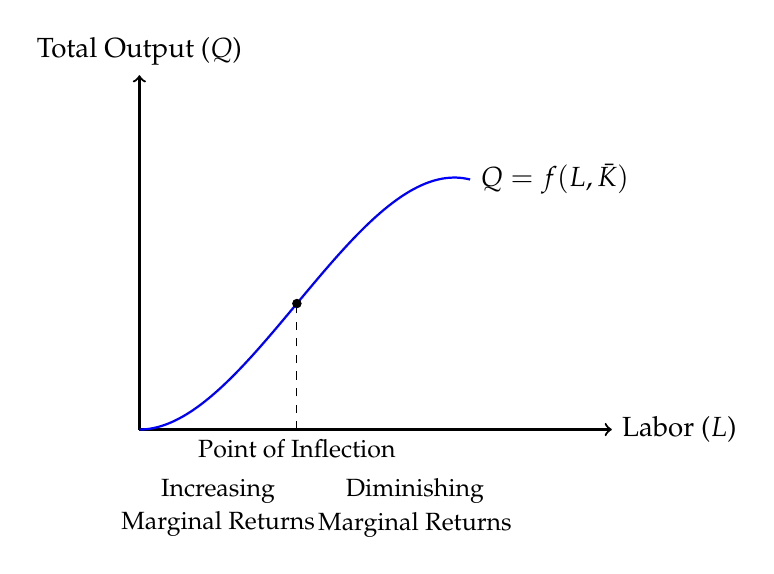
\begin{tikzpicture}[scale=1]
    % Axes
    \draw[->, thick] (0,0) -- (6,0) node[right] {Labor ($L$)};
    \draw[->, thick] (0,0) -- (0,4.5) node[above] {Total Output ($Q$)};
    
    % Production Function Curve (Cubic: Q = -0.1*L^3 + 0.6*L^2)
    % Max is at L=4, Q=3.2. Inflection is at L=2, Q=1.6
    \draw[thick, blue, smooth, domain=0:4.2, samples=100] plot (\x, {-0.1*\x*\x*\x + 0.6*\x*\x}) node[right, black] {$Q = f(L, \bar{K})$};
    
    % Indicate phases
    \draw[dashed] (2,0) node[below] {\small Point of Inflection} -- (2,1.6);
    \filldraw[black] (2,1.6) circle (1.5pt);
    \node[align=center, below] at (1,-0.5) {\small Increasing \\ \small Marginal Returns};
    \node[align=center, below] at (3.5,-0.5) {\small Diminishing \\ \small Marginal Returns};
\end{tikzpicture}
\end{center}

\textbf{Description of the Curve}: The curve initially rises at an increasing rate (increasing slope), then continues to rise but at a decreasing rate (decreasing slope), and ultimately flattens out (the slope approaches zero).

\textbf{Why does it flatten out?} \\
This is caused by the \textbf{Law of Diminishing Marginal Returns}. When at least one input (usually capital, like a facility or equipment) is held fixed, continuously adding more units of a variable input (like labor) will eventually result in smaller and smaller additions to total output (the marginal product of labor declines). Eventually, adding more labor yields almost zero additional output, causing the total production curve to flatten out.

\textbf{Example of the phenomenon}: \\
\textit{Example in a hospital ward}: The number of beds in a hospital ward is fixed (capital). Initially, hiring a few more nurses (labor) can significantly increase the quality of care and the number of patients that can be effectively treated. However, once the number of nurses reaches a very high level, all the beds are fully occupied and utilized. At this point, hiring one more nurse cannot increase the number of patients treated because the physical number of beds has become an absolute bottleneck. The total number of treated patients stops growing, and the production function flattens out.

% \clearpage
\section*{4. Consider a firm maximizing profits. We will use isoquants and isocost curves to model firm decisions. Consider a production function $Q$, such that $Q=K^{0.5}L^{0.5}$, and a cost function such that $C=wL+rK$.}

\textbf{Sketch the isoquant for Q=100 (1 point)}
\begin{itemize}[leftmargin=*]
    \item \textbf{Calculation}: Substitute $Q=100$ into the production function: $100 = K^{0.5}L^{0.5} \implies 10,000 = K \cdot L \implies K = \frac{10,000}{L}$.
    \item \textbf{Sketch Description}: This is a convex curve bowing toward the origin (a rectangular hyperbola) in the L-K coordinate system. Representative points on this curve include $(L=100, K=100)$ and $(L=50, K=200)$.
\end{itemize}
\begin{center}
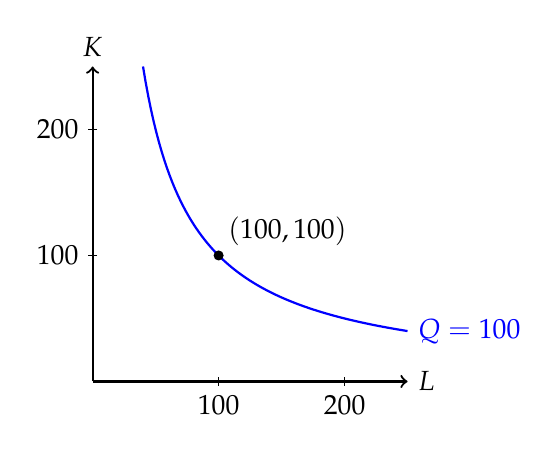
\begin{tikzpicture}[scale=0.8]
    \draw[->, thick] (0,0) -- (5,0) node[right] {$L$};
    \draw[->, thick] (0,0) -- (0,5) node[above] {$K$};
    \draw[thick, blue, domain=0.8:5, samples=100] plot (\x, {4/\x}) node[right] {$Q=100$};
    \filldraw[black] (2,2) circle (2pt) node[anchor=south west] {$(100, 100)$};
    \foreach \x/\xtext in {2/100, 4/200} \draw (\x,2pt) -- (\x,-2pt) node[below] {$\xtext$};
    \foreach \y/\ytext in {2/100, 4/200} \draw (2pt,\y) -- (-2pt,\y) node[left] {$\ytext$};
\end{tikzpicture}
\end{center}

\textbf{Sketch the isoquant for Q=200 (0.5 point)}
\begin{itemize}[leftmargin=*]
    \item \textbf{Calculation}: Substitute $Q=200$ into the production function: $200 = K^{0.5}L^{0.5} \implies 40,000 = K \cdot L \implies K = \frac{40,000}{L}$.
    \item \textbf{Sketch Description}: This curve has the same shape as the $Q=100$ isoquant but lies completely to its upper right, representing a higher level of output. A representative point is $(L=200, K=200)$.
\end{itemize}
\begin{center}
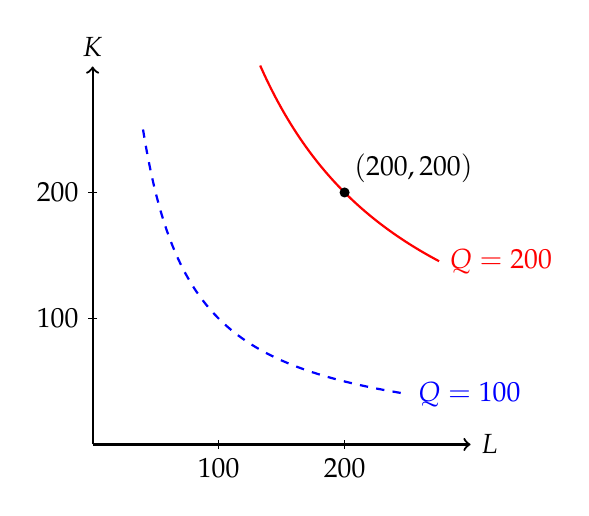
\begin{tikzpicture}[scale=0.8]
    \draw[->, thick] (0,0) -- (6,0) node[right] {$L$};
    \draw[->, thick] (0,0) -- (0,6) node[above] {$K$};
    \draw[thick, blue, dashed, domain=0.8:5, samples=100] plot (\x, {4/\x}) node[right] {$Q=100$};
    \draw[thick, red, domain=2.66:5.5, samples=100] plot (\x, {16/\x}) node[right] {$Q=200$};
    \filldraw[black] (4,4) circle (2pt) node[anchor=south west] {$(200, 200)$};
    \foreach \x/\xtext in {2/100, 4/200} \draw (\x,2pt) -- (\x,-2pt) node[below] {$\xtext$};
    \foreach \y/\ytext in {2/100, 4/200} \draw (2pt,\y) -- (-2pt,\y) node[left] {$\ytext$};
\end{tikzpicture}
\end{center}

\textbf{If $w=1$ and $r=1$, draw the isocost curve for a budget of 200. (1 point)}
\begin{itemize}[leftmargin=*]
    \item \textbf{Calculation}: Substituting the values, the isocost equation is $200 = 1 \cdot L + 1 \cdot K \implies K = 200 - L$.
    \item \textbf{Sketch Description}: This is a straight, downward-sloping line. The L-intercept (horizontal axis) is $L=200$, and the K-intercept (vertical axis) is $K=200$. The slope of the line (representing the negative of the input price ratio) is $-w/r = -1$.
\end{itemize}
\begin{center}
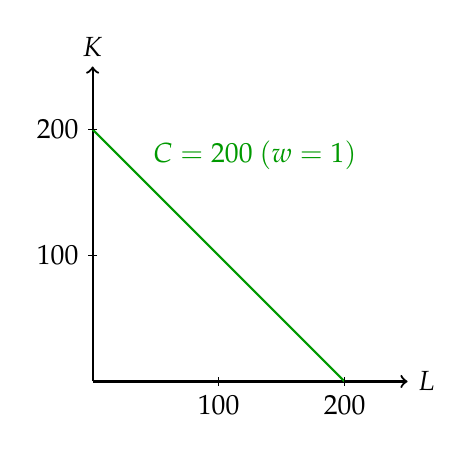
\begin{tikzpicture}[scale=0.8]
    \draw[->, thick] (0,0) -- (5,0) node[right] {$L$};
    \draw[->, thick] (0,0) -- (0,5) node[above] {$K$};
    \draw[thick, green!60!black] (0,4) -- (4,0) node[pos=0.2, above right] {$C=200\ (w=1)$};
    \foreach \x/\xtext in {2/100, 4/200} \draw (\x,2pt) -- (\x,-2pt) node[below] {$\xtext$};
    \foreach \y/\ytext in {2/100, 4/200} \draw (2pt,\y) -- (-2pt,\y) node[left] {$\ytext$};
\end{tikzpicture}
\end{center}

\textbf{If $w=2$ and $r=1$, draw the isocost curve for a budget of 200. (1 point)}
\begin{itemize}[leftmargin=*]
    \item \textbf{Calculation}: With the new prices, the isocost equation becomes $200 = 2 \cdot L + 1 \cdot K \implies K = 200 - 2L$.
    \item \textbf{Sketch Description}: This straight line is steeper than the previous one. The K-intercept remains at $K=200$, but the L-intercept rotates inward to $L=100$. The slope of the line is $-w/r = -2$.
\end{itemize}
\begin{center}
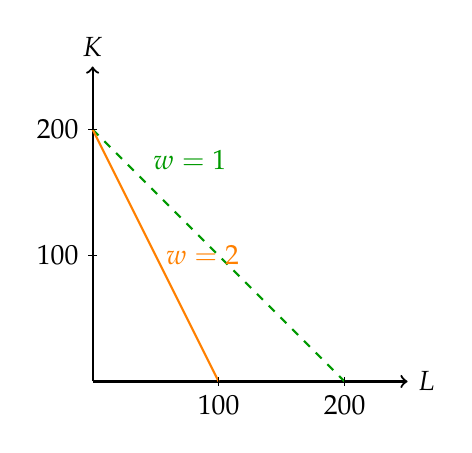
\begin{tikzpicture}[scale=0.8]
    \draw[->, thick] (0,0) -- (5,0) node[right] {$L$};
    \draw[->, thick] (0,0) -- (0,5) node[above] {$K$};
    \draw[thick, green!60!black, dashed] (0,4) -- (4,0) node[pos=0.2, above right] {$w=1$};
    \draw[thick, orange] (0,4) -- (2,0) node[pos=0.5, right] {$w=2$};
    \foreach \x/\xtext in {2/100, 4/200} \draw (\x,2pt) -- (\x,-2pt) node[below] {$\xtext$};
    \foreach \y/\ytext in {2/100, 4/200} \draw (2pt,\y) -- (-2pt,\y) node[left] {$\ytext$};
\end{tikzpicture}
\end{center}

\textbf{Find the optimal choice of K and L graphically only for the firm using the isoquant (Q) = 100 and isocost (C) = 200 curves. (1 point)}
\begin{itemize}[leftmargin=*]
    \item \textbf{Graphical Method}: The optimal choice for minimizing cost for a given output (or maximizing output for a given cost) occurs \textbf{at the point of tangency between the isoquant and the isocost curve}. At this point, the slopes of the two curves are equal, meaning the Marginal Rate of Technical Substitution ($MRTS$) equals the input price ratio ($w/r$).
    \item \textbf{Calculation}:
        \begin{itemize}[leftmargin=1.5em]
            \item Slope of the isocost curve ($w=1, r=1$) is $w/r = 1$ in absolute value.
            \item $MRTS = \frac{MP_L}{MP_K} = \frac{0.5 K^{0.5} L^{-0.5}}{0.5 K^{-0.5} L^{0.5}} = \frac{K}{L}$.
            \item Setting them equal for the point of tangency: $\frac{K}{L} = 1 \implies K = L$.
            \item Substitute $K=L$ into the $Q=100$ isoquant: $100 = \sqrt{K \cdot K} = K \implies K=100$. Thus, $L=100$.
        \end{itemize}
    \item \textbf{Conclusion}: Graphically, the unique point where the $Q=100$ curve is tangent to the $C=200$ isocost line is at \textbf{$(L=100, K=100)$}.
\end{itemize}
\begin{center}
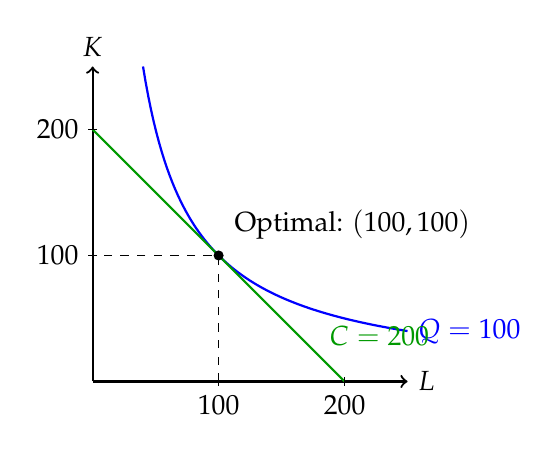
\begin{tikzpicture}[scale=0.8]
    \draw[->, thick] (0,0) -- (5,0) node[right] {$L$};
    \draw[->, thick] (0,0) -- (0,5) node[above] {$K$};
    \draw[thick, blue, domain=0.8:5, samples=100] plot (\x, {4/\x}) node[right] {$Q=100$};
    \draw[thick, green!60!black] (0,4) -- (4,0) node[pos=0.9, above right] {$C=200$};
    \filldraw[black] (2,2) circle (2pt);
    \draw[dashed] (2,0) -- (2,2) -- (0,2);
    \node[anchor=south west] at (2.1, 2.1) {Optimal: $(100, 100)$};
    \foreach \x/\xtext in {2/100, 4/200} \draw (\x,2pt) -- (\x,-2pt) node[below] {$\xtext$};
    \foreach \y/\ytext in {2/100, 4/200} \draw (2pt,\y) -- (-2pt,\y) node[left] {$\ytext$};
\end{tikzpicture}
\end{center}

\section*{5. A dental clinic employs a hygienist who works an 8-hour shift and uses a cleaning tool purchased for \$10,000.  The hygienist can treat 12 patients per shift and earns \$30 per hour. The hygienist exhibits diminishing marginal productivity throughout the course of the shift. For simplicity, assume that all patients are identical.}

\textbf{Given Information}:
\begin{itemize}[leftmargin=*, noitemsep]
    \item Labor ($L$): 8 hours per shift.
    \item Total Fixed Cost ($TFC$): \$10,000 (cleaning tool).
    \item Total Output ($Q$): 12 patients per shift.
    \item Wage rate ($w$): \$30 per hour.
    \item Total Variable Cost ($TVC$): $\$30/\text{hr} \times 8\text{ hrs} = \$240$.
\end{itemize}

\textbf{What is the average product for this hygienist? (1 point)} \\
Average Product ($AP$) = Total Output ($Q$) / Labor Input ($L$) \\
\textbf{Answer}: $AP = 12 \text{ patients} / 8 \text{ hours} = \textbf{1.5 patients per hour}$.

\textbf{What is the average variable cost of the hygienist per patient? Show your work. (1 point)} \\
Average Variable Cost ($AVC$) = Total Variable Cost ($TVC$) / Total Output ($Q$) \\
\textbf{Show your work}: $TVC = \text{Wage rate} \times \text{Hours worked} = \$30 \times 8 = \$240$. \\
$AVC = \$240 / 12 \text{ patients} = \textbf{\$20 per patient}$.

\textbf{What is the average total cost of the hygienist per patient? Show your work. (1 point)} \\
Average Total Cost ($ATC$) = Total Cost ($TC$) / Total Output ($Q$) \\
\textbf{Show your work}: Total Cost ($TC$) = Total Fixed Cost ($TFC$) + Total Variable Cost ($TVC$) = $\$10,000 + \$240 = \$10,240$. \\
$ATC = \$10,240 / 12 \text{ patients} = \textbf{\$853.33 per patient}$ (rounded to nearest cent).

\textbf{Based only on the information above, it can be assumed that the Hygienist will spend more than \underline{\hspace{1cm}} minutes treating their final patient of the day. Show your work and briefly explain. Name the principle driving your answer. (2 points)} \\
Answer: \textbf{40} (minutes). \\
\textbf{Show your work and briefly explain}: An 8-hour shift equals 480 minutes. The simple arithmetic average time spent per patient is $480 \text{ minutes} / 12 \text{ patients} = 40 \text{ minutes per patient}$. However, the problem states that the hygienist exhibits \textbf{diminishing marginal productivity} throughout the shift. This implies that as the shift goes on, the hygienist becomes more tired or less efficient, and treating each subsequent patient takes progressively more time than the previous one. Because the times are increasing but must average exactly 40 minutes overall, the time spent on the very last patient of the day must be strictly greater than the overall average of 40 minutes. \\
\textbf{Name the principle}: \textbf{The Law of Diminishing Marginal Returns} (or Diminishing Marginal Productivity).

\section*{6. For the next two questions, assume patients 1-3 take 20 min each, patients 4-6 take 30 min each, patients 7-8 take 40 min each, patients 9-10 take 50 min each, patient 11 takes 70 min, and patient 12 takes 80 min.}

\textbf{What is the marginal cost of the hygienist for the 6th patient? (1 point)} \\
The given time for the 6th patient is 30 minutes. \\
\textbf{Calculation}: $MC_{\text{6th patient}} = 30 \text{ minutes} \times \$0.50/\text{minute} = \textbf{\$15}$.

\textbf{What is the marginal cost of the hygienist for the 7th patient? (2 point)} \\
The given time for the 7th patient is 40 minutes. \\
\textbf{Calculation}: $MC_{\text{7th patient}} = 40 \text{ minutes} \times \$0.50/\text{minute} = \textbf{\$20}$.

\end{document}
